\documentclass[10pt]{beamer}

\usetheme[progressbar=frametitle]{metropolis}
\usepackage{appendixnumberbeamer}
\usepackage{lipsum}
\usepackage{amsmath}
\usepackage{amssymb}
\usepackage{mathtools}
\usepackage{booktabs}
\usepackage{hyperref}
\usepackage[scale=2]{ccicons}
\usepackage{pgfplots}
\usepgfplotslibrary{dateplot}
\usepackage{dirtytalk}
\usepackage{xspace}
\usepackage{fancybox}
\usepackage{enumerate}
\usepackage[ruled,vlined]{algorithm2e}
\usepackage{algorithmic}
\usepackage{tikz}
\usepackage{xcolor}
\usepackage{lipsum}
\usepackage{graphicx}
\usepackage{mwe} % for blindtext and example-image-a in example
\usepackage{wrapfig}
\allowdisplaybreaks
\newcommand{\themename}{\textbf{\textsc{metropolis}}\xspace}
\newcommand*\circled[1]{\tikz[baseline=(char.base)]{
    \node[shape=circle,draw,inner sep=2pt] (char) {\#1};}}

\usepackage[backend=bibtex,
natbib=true]{biblatex}

\bibliography{reference} 

\DeclarePairedDelimiter\ceil{\lceil}{\rceil}
\DeclarePairedDelimiter\floor{\lfloor}{\rfloor}
\newcommand{\Cross}{\mathbin{\tikz [x=1.1ex,y=1.1ex,line width=.1ex] \draw (0,0) -- (1,1) (0,1) -- (1,0);}}%
\hypersetup{
    colorlinks=true,
    linkcolor=blue,
    filecolor=magenta,
    urlcolor=cyan,
    citecolor=magenta, 
}
\definecolor{mpigreen}{HTML}{005f79}
\setbeamercolor{frametitle}{bg=mpigreen}

\title{The dynamic vehicle routing problem with stochastic customer requests and multiple delivery routes}

\author{Lorenzo Sciandra, \and Stefano Vittorio Porta, \and \newline Jean-François Côté\\}
\date{A.A. 2021-2022}
\institute{Università degli Studi di Torino}
\titlegraphic{\vspace{4.5cm}\flushright
\includegraphics[width=2.2cm,height=2.2cm]{Images/LOGO_UNITO_VERTICALE_COLORE.png}} %\logo{
\includegraphics[scale=0.15]{Images/LOGO_UNITO_VERTICALE_COLORE.png}}


\hypersetup{colorlinks,linkcolor=,urlcolor=red}
\setbeamertemplate{section in toc}{\inserttocsectionnumber.~\inserttocsection}




\begin{document}

    \maketitle

    \section*{Indice Argomenti}\label{sec:indice-argomenti}

    \begin{frame}{Indice argomenti}
        \tableofcontents
    \end{frame}
    
    \section{Definizione del Problema}\label{sec:def-problema}

    \begin{frame}{Problema Dinamico}
        Matematicamente il problema è definibile con un grafo diretto {\(G = (L \cup \{ 0\},A)\)} dove {\(L\)} è l\textquotesingle insieme dei nodi o posizioni possibili dei \textbf{clienti}, {\(0\)} è il \textbf{deposito} e {\(A\)} è l'insieme di archi con associati \textbf{tempo di viaggio} {\(t_{ij}\)} e \textbf{costo} {\(c_{ij}\)} per passare dal nodo {\(i\)} al nodo {\(j\)}. \newline Viene definito con {\(T\)} l'\textbf{orizzonte temporale} ossia le ore lavorative del deposito e quindi l'orario limite dal quale può partire un \textbf{veicolo}. \newline {\(R\)} è invece l'insieme delle \textbf{richieste dei clienti} per i quali dobbiamo caricare dal deposito gli oggetti ordinati per essere consegnati. Di queste generalmente solo poche sono conosciute fin dall'inizio dell'orizzonte temporale, la maggior parte infatti diventeranno note col procedere del tempo, questo è l'aspetto \textbf{dinamico} del problema: non tutto è conosciuto a priori.
    \end{frame}

    \begin{frame}{Problema Stocastico}  
    Ogni richiesta {\(k\)} è caratterizzata da un \textbf{release time} {\(r_{k}\)} che è il tempo nella quale questa diventa nota e da una finestra temporale per la consegna. La finestra è un intervallo {\(\lbrack e_{k},l_{k}\rbrack\)} i cui estremi rappresentano rispettivamente il primo e l'ultimo possibile tempo di arrivo per servire il cliente $k$.\newline Quando eventi futuri risultano conosciuti solo dalla loro distribuzione di probabilità, il problema viene definito \textbf{stocastico}. In questo problema distribuzioni di probabilità riguardanti il numero di clienti che chiederanno il servizio, il momento in cui lo faranno, la loro posizione e le finestre temporali sono generate usando dati di scenari passati. Ad esempio è previsto che il tasso di arrivo delle richieste future sia un processo di Poisson con parametro {\(\lambda_{i}\)} con {\(i\)} indice del luogo della richiesta.
    \end{frame}
    
    \begin{frame}{Funzione Obiettivo}  
    Per quanto riguarda la consegna abbiamo un numero finito e fisso {\(M\)} di veicoli considerati, per semplicità, con capacità illimitata. Il percorso di un veicolo inizia dal deposito, serve un certo numero di clienti e ritorna al deposito. Formalmente una route è una sequenza $[-1,r_1,...,r_n,-1]$ dove $1 \leq r_i \leq |R|$ sono le richieste tutte distinte e $-1$ rappresenta il depot. Il \textbf{costo di un percorso} è $c(p) = c_{-1,r_1} + c_{r_1,r_2}+ \cdot \cdot \cdot + c_{r_n,-1}$. \newline La funzione obiettivo è gerarchica: prima si massimizza sul numero di richieste servite e poi si minimizza sulla distanza di viaggio. 
    \end{frame}

    \begin{frame}{Piano di Instradamento}
        Un \textbf{piano di instradamento} è un insieme di routes $\{p_1,...,p_M\}$, una per ogni veicolo, che serve ogni cliente esattamente una volta. Il piano assegna ad ogni cliente un solo predecessore ed un solo successore all'interno del percorso.  Il \textbf{costo di viaggio di un piano} è la somma dei costi delle sue routes e quindi $\sum_{i=1}^M c(p_i)$. Le decisioni prese durante l'esecuzione sono basate su un \textbf{piano prescelto} che evolve nel tempo. Il piano prescelto viene selezionato da una \textbf{funzione di consenso} e tutti gli altri mantenuti devono essere consistenti con esso.
    \end{frame}

    \section{Modellazione del Problema}\label{sec:mod-problema}
    \begin{frame}{Dynamic Pickup and Delivery Problem with Time Windows and Release Dates}  
    Il problema è stato modellato come un \textbf{Dynamic Pickup and Delivery Problem with Time Windows and Release Dates}. Ogni richiesta {\(k\)} ha quindi associata una coppia di nodi {\((i,j)\)} in cui {\(i\)} è il deposito con il pickup del materiale da consegnare e {\(j\)} è il punto in cui risiede il cliente e dove dovrà avvenire quindi la consegna. Sia la raccolta che la consegna hanno associata una finestra temporale all'interno della quale l'azione dovrà avvenire e, rispettivamente si parla di {\(\lbrack r_{k},l_{k}\rbrack\)} per la raccolta al deposito e {\(\lbrack e_{k},l_{k}\rbrack\)} per la consegna al cliente.
    \end{frame}

    \begin{frame}{Event-Driven}
         Come si fa generalmente per problemi dinamici l'\textbf{ottimizzazione è event-driven}, ossia viene performata ogni volta che si hanno nuove informazioni veicolate da un nuovo evento che si è verificato nel sistema. Quando si presenta un nuovo evento si colleziona tutto ciò che si conosce e si esegue un passo di ottimizzazione che pianifica le routes da eseguire.
    \end{frame}

    \begin{frame}{Eventi}
        Gli eventi che vengono considerati sono:

        \begin{enumerate}
            \label{events}
            \item si ha una nuova richiesta nota e c'è un veicolo al deposito pronto per partire
            \item un veicolo ha finito una route e arriva al deposito
            \item un veicolo ha terminato il tempo di attesa al deposito: se le richieste note sono poche il veicolo ha infatti la possibilità di aspettare che ce ne siano un certo numero minimo per avere soluzione migliore e più robusta riguardo a ciò che dovrà accadere
            \item una consegna è stata completata. 
        \end{enumerate}
    \end{frame}

    \begin{frame}{Reoptimization}
        Ogni volta che si verifica un evento abbiamo 3 algoritmi a disposizione:

        \begin{itemize}
            \item \textbf{Reoptimization}: classico metodo usato per risolvere problemi dinamici con pseudocodice: 
                \begin{figure}[h!]
                    \centering
                    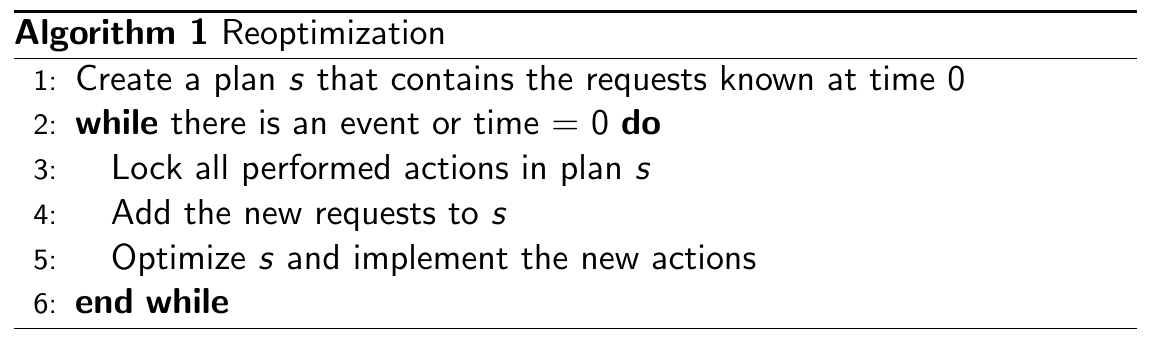
\includegraphics[scale=0.25]{Images/Reoptimization.png}
                    \caption{Reoptimization Algorithm}
                    \label{fig:reoptimization}
                \end{figure}
        \end{itemize}
    \end{frame}

    \begin{frame}{Two lookahead algorithms}
        \begin{itemize}
            \item \textbf{Two lookahead algorithms}: che cercano di anticipare le informazioni future per fare migliori pianificazioni. Questi usano scenari probabilistici con informazione stocastica campionata: nello specifico ad essere campionata è la distribuzione di probabilità che riguarda la presenza/assenza di una richiesta e il suo istante temporale. Ottimizzando gli scenari si ottengono routes, una per scenario, contententi la gestione sia di richieste note che di probabili richieste future . Ovviamente un veicolo prima di partire deve aspettare (al deposito) che queste si verifichino per sapere se caricare o meno il materiale da consegnare. I due approcci usati e uniti nel codice di Jean-François Côté sono quelli proposti in Bent e Van Hentenryck\cite{SBPPDVR} e Hvattum, Løkketangen e Laporte \cite{BRH} che andremo nel seguito a descrivere.
        \end{itemize}
    \end{frame}

  \begin{frame}{Esempio}
        \begin{figure}[h!]
            \centering
            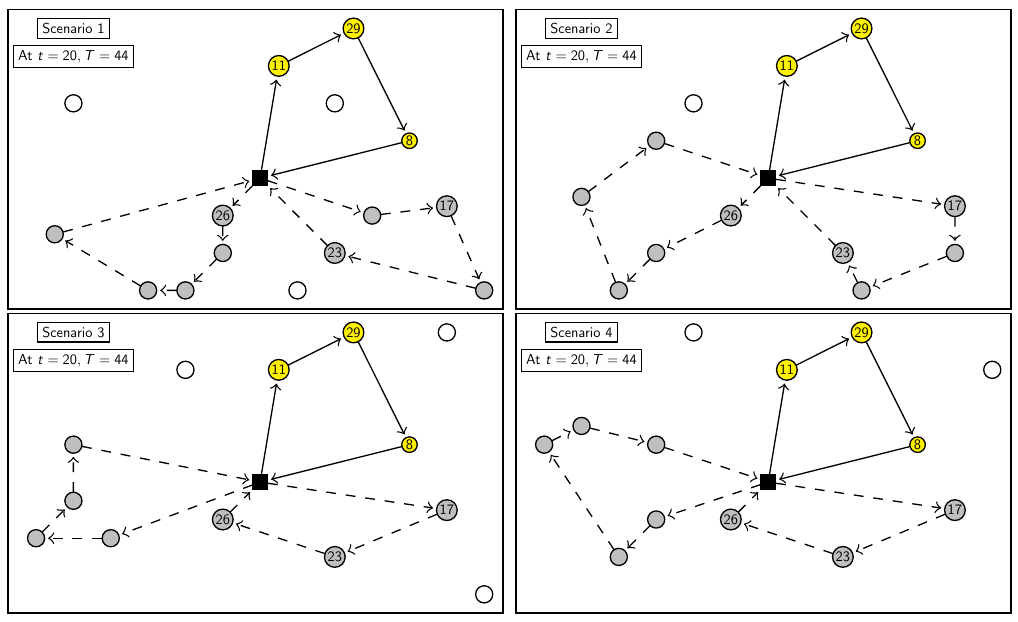
\includegraphics[scale=0.3]{Images/OptimizedScenario.png}
            \caption{Scenari Ottimizzati}
            \label{fig:optimizedScenario}
        \end{figure}
  \end{frame}


    \subsection{Scenario-Based Planning Approach}\label{sec:sbpa}
    \begin{frame}{SBPA Algorithm}
        \begin{figure}[h!]
                \centering
                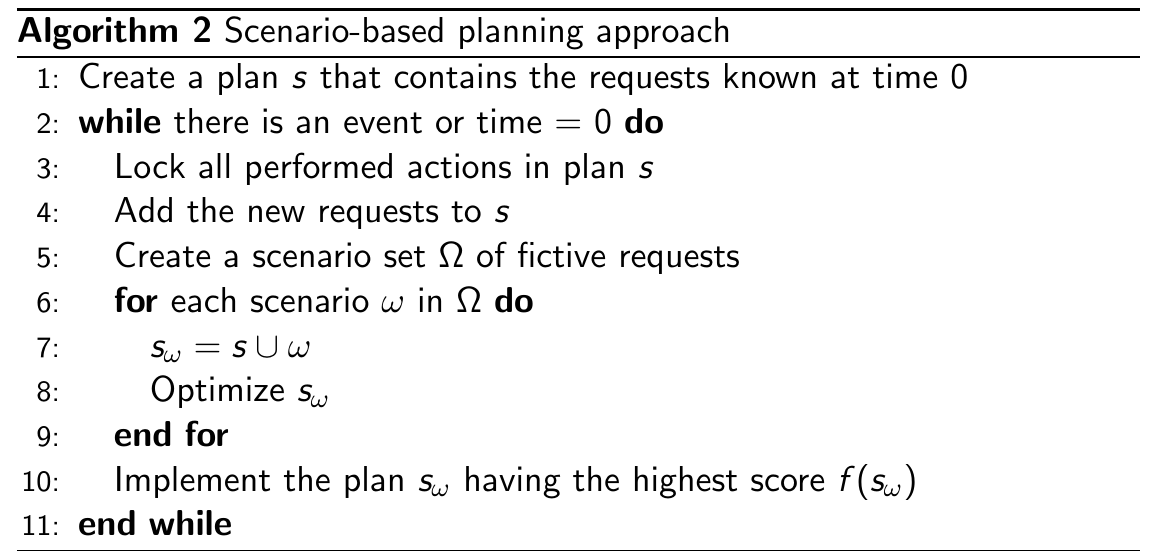
\includegraphics[scale=0.25]{Images/SBPAAlgorithm.png}
                \caption{SBPA Algorithm}
                \label{fig:reoptimization}
            \end{figure}
    \end{frame}

    \begin{frame}{Route Similarity-1}
        Nel paper \cite{SBPPDVR} si propone di scegliere come scenario finale quello che presenta il migliore score ottenuto con una certa \textbf{funzione consenso}, in questo caso mediante una \textbf{Route Similarity}. \newline Entrando nei dettagli ad ogni piano viene associato come score la somma delle volte in cui una sua route compare uguale anche nei piani ottenuti per altri scenari. In questo caso con \textit{"compare uguale"} intendiamo proprio che devono risultare le stesse richieste e nello stesso ordine. Non vengono considerate nel conteggio le route che contengono almeno una richiesta futura e per le quali dobbiamo attendere.
    \end{frame}

    \begin{frame}{Route Similarity-2}
        \begin{figure}
            \centering
            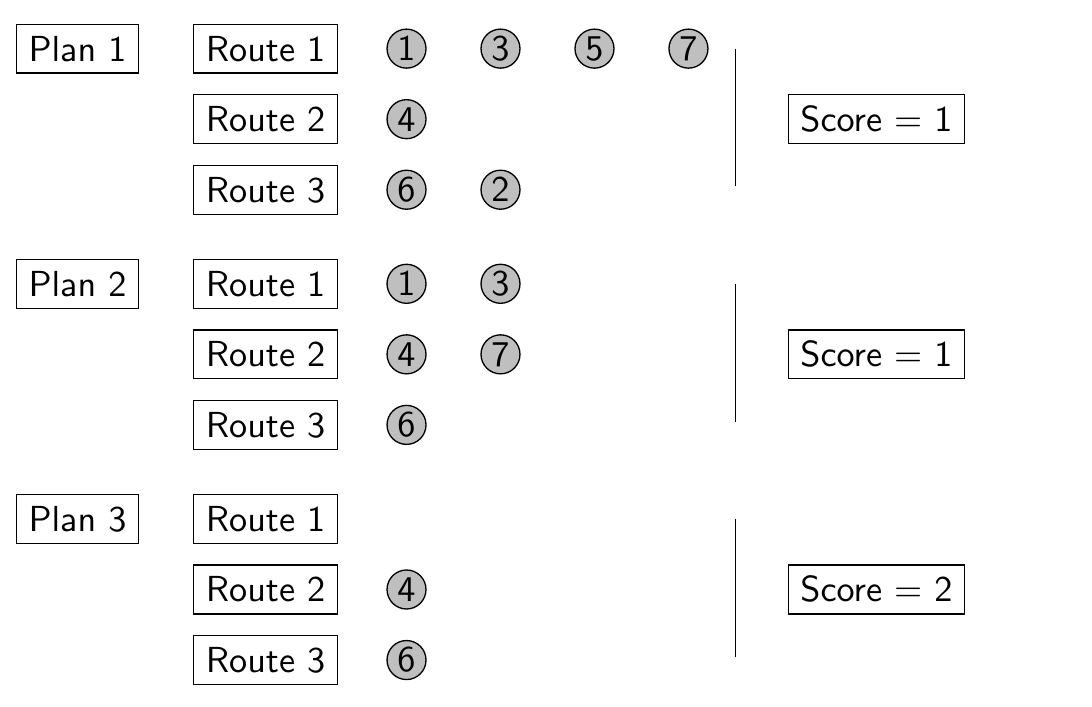
\includegraphics[scale=0.22]{Images/RouteSimilarity.png}
            \caption{Route Simalirity}
            \label{fig:RouteSimilarity}
        \end{figure}
    \end{frame} 

    \begin{frame}{Approccio Miope - Nuove Funzioni Consenso}
        Questo criterio, mostrato in \ref{fig:RouteSimilarity}, risulta però \textbf{miope} e non riesce a comprendere il trend reale che si sta verificando: sceglie sempre la strategia che richiede impegno minimo. Nello specifico quando i piani per i vari scenari sono molto diversi sarà scelto quello con meno routes e tutte molto corte, dato che avranno più probabilità (dal momento che sono composte da poche mosse) di presentarsi in altri piani. Per questo Jean-François e i suoi collaboratori hanno proposto due diverse \textbf{funzioni consenso}.
    \end{frame}

    \begin{frame}{Assigment Similarity}
        \textbf{Assignment Similarity} : lo score di ogni piano è la somma di tutti i numeri di volte in cui la coppia (richiesta, numero di route) nel piano si presenta allo stesso modo in altri piani. Questo permette di non favorire il più corto:
        \begin{figure}[h!]
            \centering
            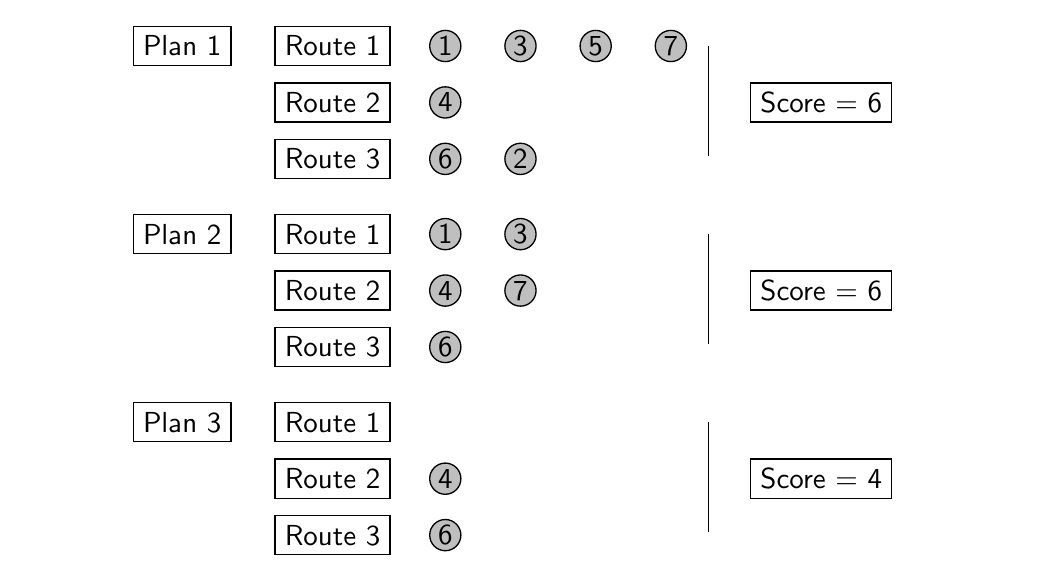
\includegraphics[scale=0.22]{Images/AssignmentSimilarity.png}
            \caption{Assignment Similarity}
            \label{fig:AssignmentSimilarity}
        \end{figure}
    \end{frame}

    \begin{frame}{Edit Distance}
        \textbf{Edit Distance}: lo score di ogni piano è la somma dei numeri di cambiamenti che necessita per essere uguale agli altri piani. In questo caso, a differenza dei precedenti, più lo score è basso meglio è:
        \begin{figure}[h!]
            \centering
            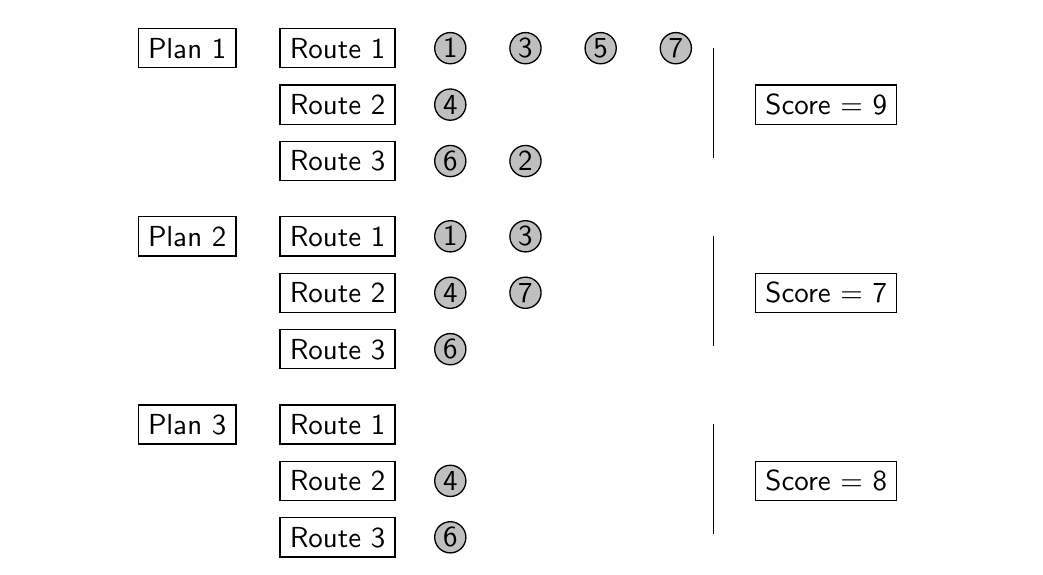
\includegraphics[scale=0.22]{Images/EditDistance.png}
            \caption{Edit Distance}
            \label{fig:EditDistance}
        \end{figure}
    \end{frame}

    \subsection{Branch \& Regret}\label{sec:b-and-r}
    \begin{frame}{Branch \& Regret -1}
        L'approccio proposto in \textcite{BRH} è simile al precedente SBPA, ma prevede alcuni passi addizionali a livello algoritmico. Nello specifico una volta ottimizzati e risolti tutti gli scenari ci si assicura, forzandole, che ogni richiesta conosciuta e reale sia servita nello stesso intervallo di tempo in tutti i piani e che in ogni piano ogni veicolo visiti le stesse richieste. Lo pseudocodice è:
        \begin{figure}[h!]
            \centering
            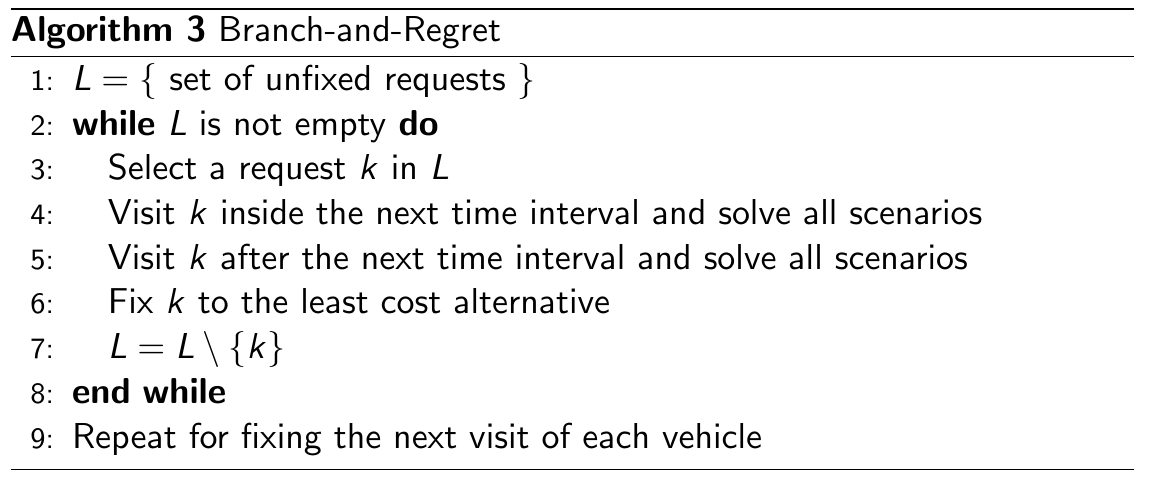
\includegraphics[scale=0.22]{Images/Branch-and-RegretAlg.png}
            \caption{B\&R algorithm}
            \label{fig:EditDistance}
        \end{figure}
    \end{frame}

    \begin{frame}{Branch \& Regret -2}
        Questo algoritmo può essere combinato, come sottoprocedura, nel precedente SBPA, inserendo la chiamata al posto del for di riga 6. Entrando nei dettagli il B\&R prende le richieste non fissate reali e va a vedere quale sarebbe la media dei costi in tutti gli scenari se ognuna di questa (una per volta) venisse gestita nella prossima route o in una delle successive. Si sceglie l'alternativa migliore e si fissa in tutti gli scenari. Una volta fatto ciò per tutte le richieste l'algortimo viene rieseguito non per fissare le richieste nelle route, ma per fissarne l'ordine. Quest'idea non si applica bene direttamente al nostro problema in questione perchè richiede che tutte le routes siano definite prima che il veicolo parta e quindi che tutto ciò che deve essere consegnato sia già caricato, ma come già accennato precedentemente, noi vorremmo aspettare che le richieste si verifichino.
    \end{frame}

    \subsubsection{Diverso Schema di Branch}\label{sec:b-and-r-branchschema}
    \begin{frame}{Diverso Schema di Branch-1}
        Nel B\&R la fase di \textbf{Branch} consiste nel scegliere se una certa richiesta vada gestita ora o in futuro, mentre la fase di \textbf{Regret} consiste nel fissare l'alternativa con il costo più conveniente. Per adattarlo all'esigenze del problema in questione Jean-François e i suoi colleghi hanno proposto un diversa fase di braching con schema:
        \begin{itemize}
            \item \textbf{go\_now}: se la richiesta {\(k\)} farà parte di una route che parte ora
            \item \textbf{wait}: se la richiesta {\(k\)} sarà assegnata ad una route che partirà dopo
            \item \textbf{reject}: se la richiesta {\(k\)} non sarà servita
        \end{itemize}
         Un possibile albero generato dal B\&R può essere il seguente:
    \end{frame}

    \begin{frame}{Diverso Schema di Branch-2}
    \noindent\begin{minipage}{0.3\textwidth}
        \begin{figure}[h!]
            \centering
            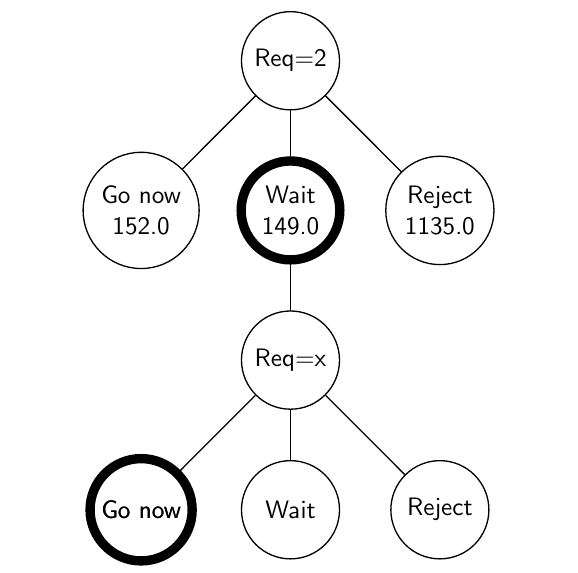
\includegraphics[scale=0.2]{Images/Branch-And-Regret-View.png}
            \caption{Branch \& Regret View}
            \label{fig:Branch-and-RegretView}
        \end{figure}
        \end{minipage}%
        \hfill%
        \begin{minipage}{0.6\textwidth}
            Tra tutte le richieste non servite viene scelta la {\(k=2\)} che sarà gestita con l'azione che presenta costo minimo tra tutti i piani, in questo caso \textbf{wait}. La richiesta immediamente successiva $x$ può invece portare ad un costo complessivo minimo se gestita immediatamente. Il processo di ottimizzazione procede in questo e viene stoppato quando tutti i piani implementano le stesse alternative di gestione di ogni richiesta reale. A questo punto viene selezionato un piano con una delle 3 funzioni consenso prima definite.
        \end{minipage}
    \end{frame}

    \section{Branch \& Bound}\label{sec:branch-and-bound}
    \begin{frame}{Basi Implementative}
        Ovviamente per poter sviluppare il nostro algoritmo si è resa necessaria l'implementazione di una nuova classe dedicata all'ottimizzazione mediante Branch \& Bound, basandoci anche su parte delle API già presenti nel progetto, senza le quali sarebbe stato necessario un lavoro molto più a basso livello. In questo caso invece, ci siamo potuti concentrare su strutture dati e algoritmi ad alto livello, permettendo uno sviluppo, testing e debugging più rapido e semplice, anche grazie all'adozione di linee guida e pattern suggeriti anche da Jean-François.
    \end{frame}

    \begin{frame}{Ottimizzatore}
        L'algoritmo viene richiamato all'interno di una funzione wrapper $\texttt{Optimize()}$ spesso implementata da Jean-François nella sua libreria per guidare tutto il processo ottimizzatorio e di simulazione a partire dall'istanziazione iniziale delle variabili necessarie per proseguire con la gestione di ogni evento lungo tutto l'orizzonte temporale e la stampa finale dei risultati. Esattamente come prima indicato a livello teorico, al verificarsi di ogni evento saranno generati $n$ scenari e ottimizzati. L'ottimizzatore sfrutta un'implementazione dell'ALNS \cite{Ropke} sviluppata da Jean-François che effettua un numero di iterazioni di distruzione e ricostruzione parziale dei percorsi generati in modo da cercare di ottimizzarli. Il numero di iterazioni è specificato da un parametro impostato prima dell'inizio della ricerca di soluzioni.
    \end{frame}

    \begin{frame}{Branch \& Bound}
        Abbiamo realizzato il Branch \& Bound sia in versione iterativa che ricorsiva e a loro volta entrambe sia in versione Best-First che Depth-First. Tutte le versioni sono void e la migliore soluzione intera si troverà, alla fine dell'esecuzione, nello spazio di memoria puntato dal puntatore passato in input. Per spiegare correttamente il Branch \& Bound dividiamolo nelle sue parti fondamentali.
    \end{frame}

    \subsection{Branching}\label{sec:branching}
    \begin{frame}{Branching-1}
        Preso un certo nodo dell'albero delle decisioni i suoi figli vengono ottenuti, all'inizio della procedura, con la chiamata a \texttt{GetNextActionDecisions()}. Quest'ultima funzione andrà ad assegnare il vettore \texttt{current\_decisions} con una triplice versione della decisione selezionata una per ogni tipo di azione che possiamo performare su di essa: \textit{go\_now, wait, don't deliver}. Se questo vettore è vuoto vuol dire che abbiamo già analizzato tutte le possibilità per tutte le richieste reali per ora note e possiamo terminare, aggiornando eventualmente la miglior soluzione trovata con quella corrente. 
    \end{frame}

    \begin{frame}{Branching-2}
        Nel caso invece in cui ci sia ancora almeno una richiesta reale da analizzare andiamo ad ottimizzare ogni scenario forzando in ognuno di essi tutte le decisioni precedentemente prese insieme a quella nuova corrente da considerare. E' importante quindi mantenere un vettore di \texttt{working\_decisions} che vada aggiornato mano a mano che una richiesta è gestita. Si andranno quindi a generare i nuovi nodi, figli della \texttt{current\_decision} che saranno immediatamente esplorati nel caso Dept-First ed inseriti nella lista dei nodi da esplorare nel caso Best-First. A dire il vero entrambe le visite sono gestite con coda con la sola differenza che per la prima questa è semplicemente una LIFO, mentre per la seconda deve essere ordinata ogni volta che vengono inseriti nuovi nodi.
    \end{frame}

    \subsection{Bounding}\label{sec:bounding}
    \begin{frame}{Bounding}
        La fase di bounding permette di evitare parte dell'esplorazione dell'albero. Nello specifico, prima di fare la chiamata ricorsiva su un nodo, o equivalentemente prima di espanderlo ed inserire i figli nella lista nella versione iterativa, ci si accerta che abbia un costo medio su tutti gli scenari minore dell'ottimo finora trovato e possa quindi migliorare la nostra soluzione corrente.
    \end{frame}

    \subsection{Best-First vs Depth-First}\label{sec:bf-vs-df}
    \begin{frame}{Best-First vs Depth-First}
        L'albero generato dal B\&B può essere esplorato in due modi diversi, il cui controllo avviene tramite un parametro globale dell'ottimizzazione che permette di scegliere un'\textbf{esplorazione in profondità} oppure una \textbf{Best First}. Entrambe sono realizzate con una lista di nodi con la sola differenza che il primo approccio prevede di usarla in maniera LIFO, mentre il secondo inserisce ed estrae i nodi da esplorare in accordo con il loro valore di costo medio. C'è da precisare il fatto che nel caso nella versione ricorsiva questo non porta ad un approccio Best-First globale, complessivo di tutte le richieste nell'albero, come invece accade per la versione iterativa. Quello che si origina è invece una Best-First a livello in cui ogni padre decide prima di esplorare i figli più promettenti. Questo verrà chiarito con un paio di esempi di esecuzione.
    \end{frame}

    \section{Risultati}\label{sec:risultati}
    \begin{frame}{Output}
        Per accorgerci dell'eventuale differenza di piano ottimo restituito dal Branch \& Regret rispetto a quello reale trovato con il Branch \& Bound abbiamo deciso di stampare, durante la generazione dell'albero, comandi \href{https://graphviz.org/}{Graphviz} che ci permettessero di visulizzare graficamente la situazione. Ci spieghiamo meglio. 
    \end{frame}

    \begin{frame}{BBNode}
        Per fare questo abbiamo definito una classe di supporto $\texttt{BBNode}$ (Branch\&Bound Node) che contiene tutte le informazioni rilevanti riguardo alla posizione di un nodo nell'albero: 
        \begin{itemize}
            \item ID univoco del nodo
            \item ID della richiesta considerata
            \item ID del nodo genitore
            \item Tipo di decisione che il nodo rappresenta
            \item Costo raggiunto per poter svolgere la decisione correlata al nodo
            \item Puntatori ai BBNode figli
        \end{itemize}
        Una volta generato completamente tutto l'albero, che sarà un vettore di $\texttt{BBNode}$, viene post-processato aggiungendo ad ogni nodo informazioni booleane riguardo l'appartenenza al percorso ottimo e a quello definito dal B\&R. A questo punto ciclando sul vettore si stampa per ogni nodo la dichiarazione del nodo stesso e l'arco che lo collega univocamente al padre. Mostriamo alcuni esempi.
    \end{frame}

    \begin{frame}{BB e BR con stessa path}
            \begin{figure}[!h]
                \centering
                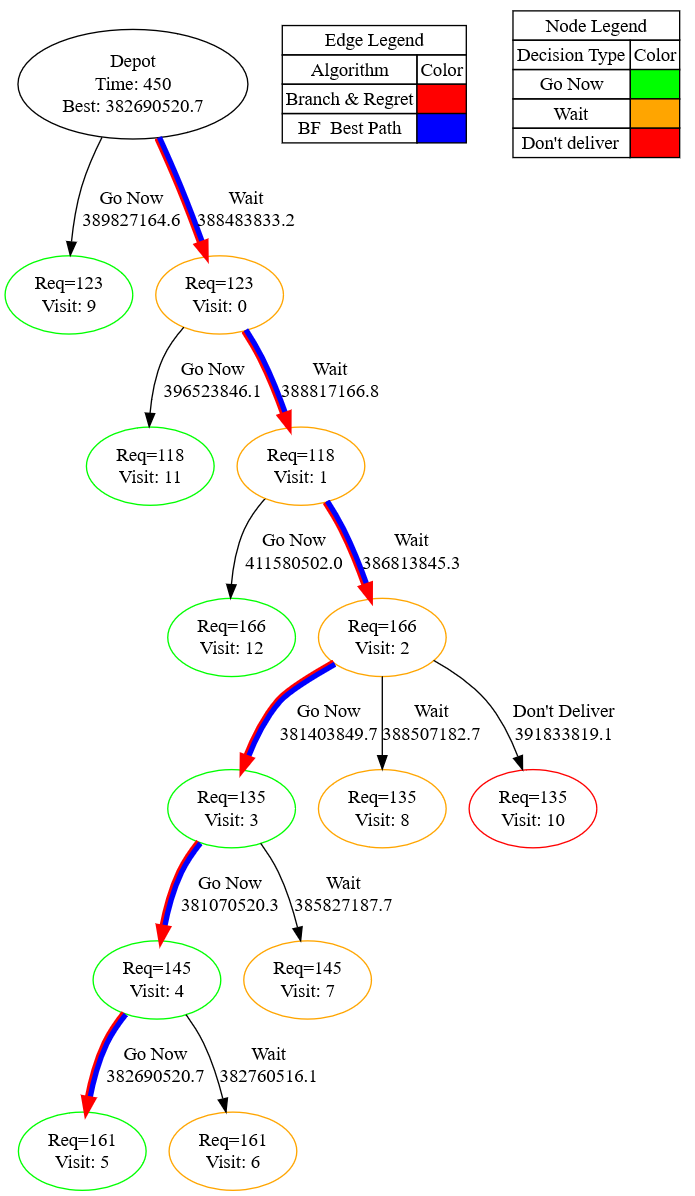
\includegraphics[width=0.37\textwidth]{Images/same_path.png}
                \caption{B\&B Best-First e B\&R scelgono lo stesso percorso}
            \label{fig:BBBFuguale}
            \end{figure}
    \end{frame}

    \begin{frame}{BB Best-First vs BR}
        \begin{figure}[h!]
            \centering
            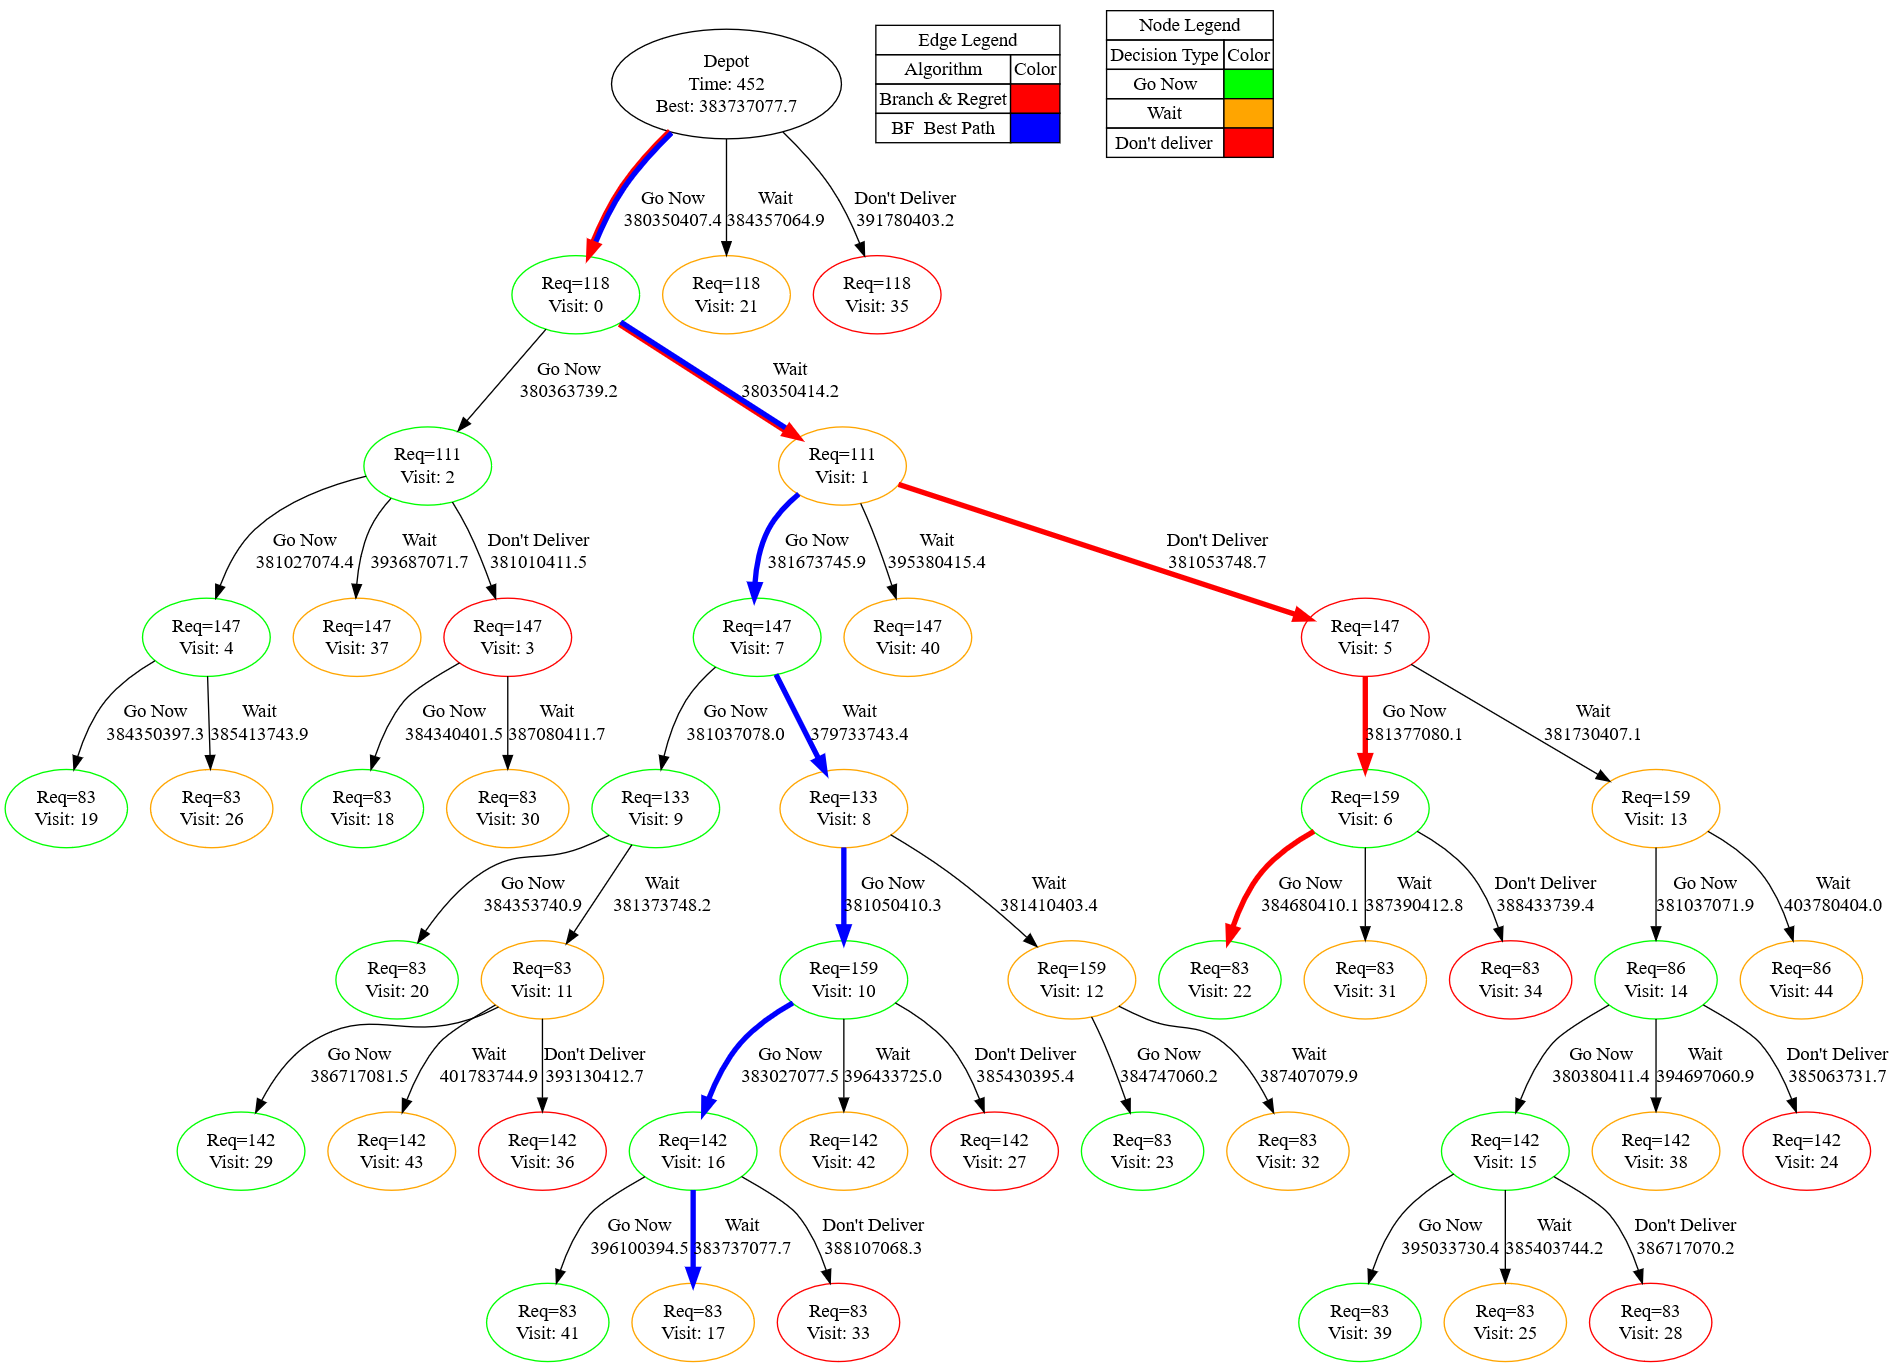
\includegraphics[width=0.85\textwidth]{Images/omg.png}
            \caption{B\&B Best-First trova un percorso migliore del B\&R}
        \label{fig:BBBFmigliore}
        \end{figure}
    \end{frame}

    \begin{frame}{BB Best-First doppio percorso ottimo}
        \begin{figure}[h!]
            \centering
            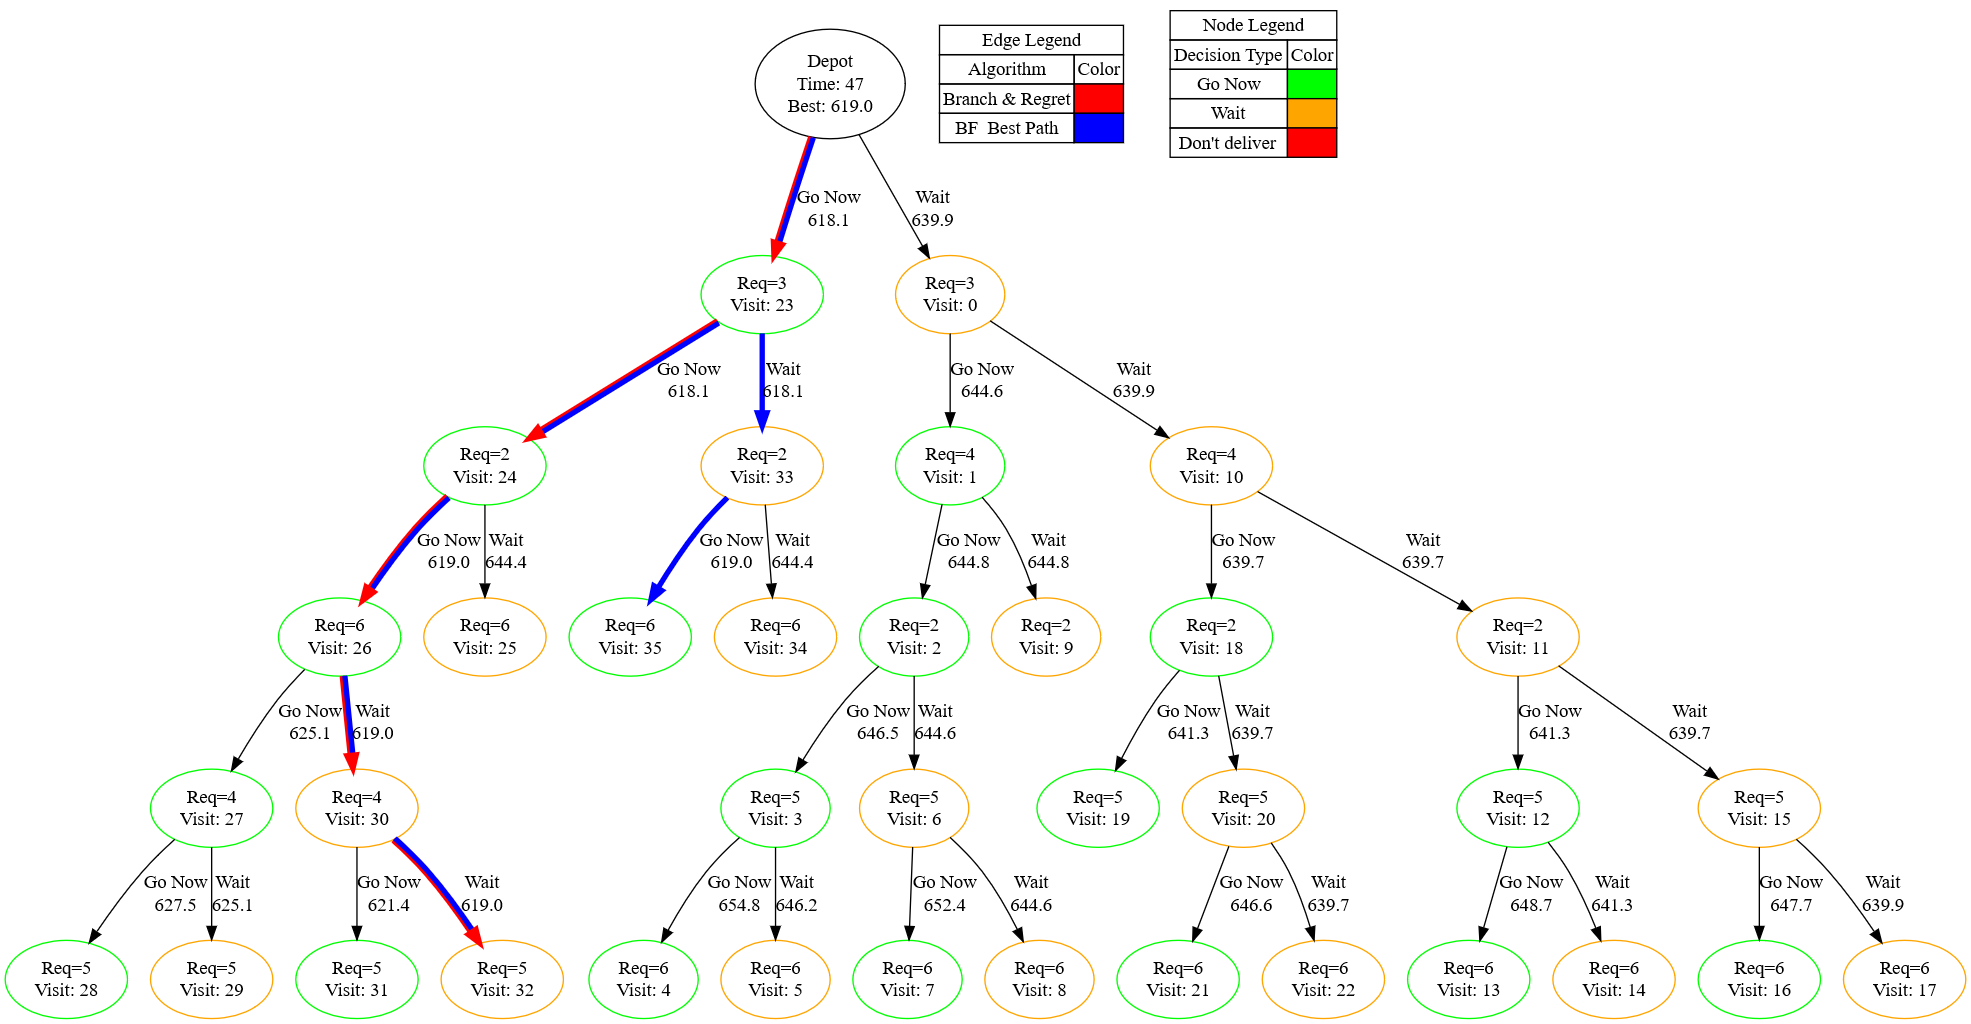
\includegraphics[width=1\textwidth]{Images/raro.png}
            \caption{B\&B trova due percorsi ottimi di uguale costo}
            \label{fig:BBBFduepath}
        \end{figure}
    \end{frame}

    \begin{frame}{BB Depth-First vs BR}
           \begin{figure}[h!]
                \centering
                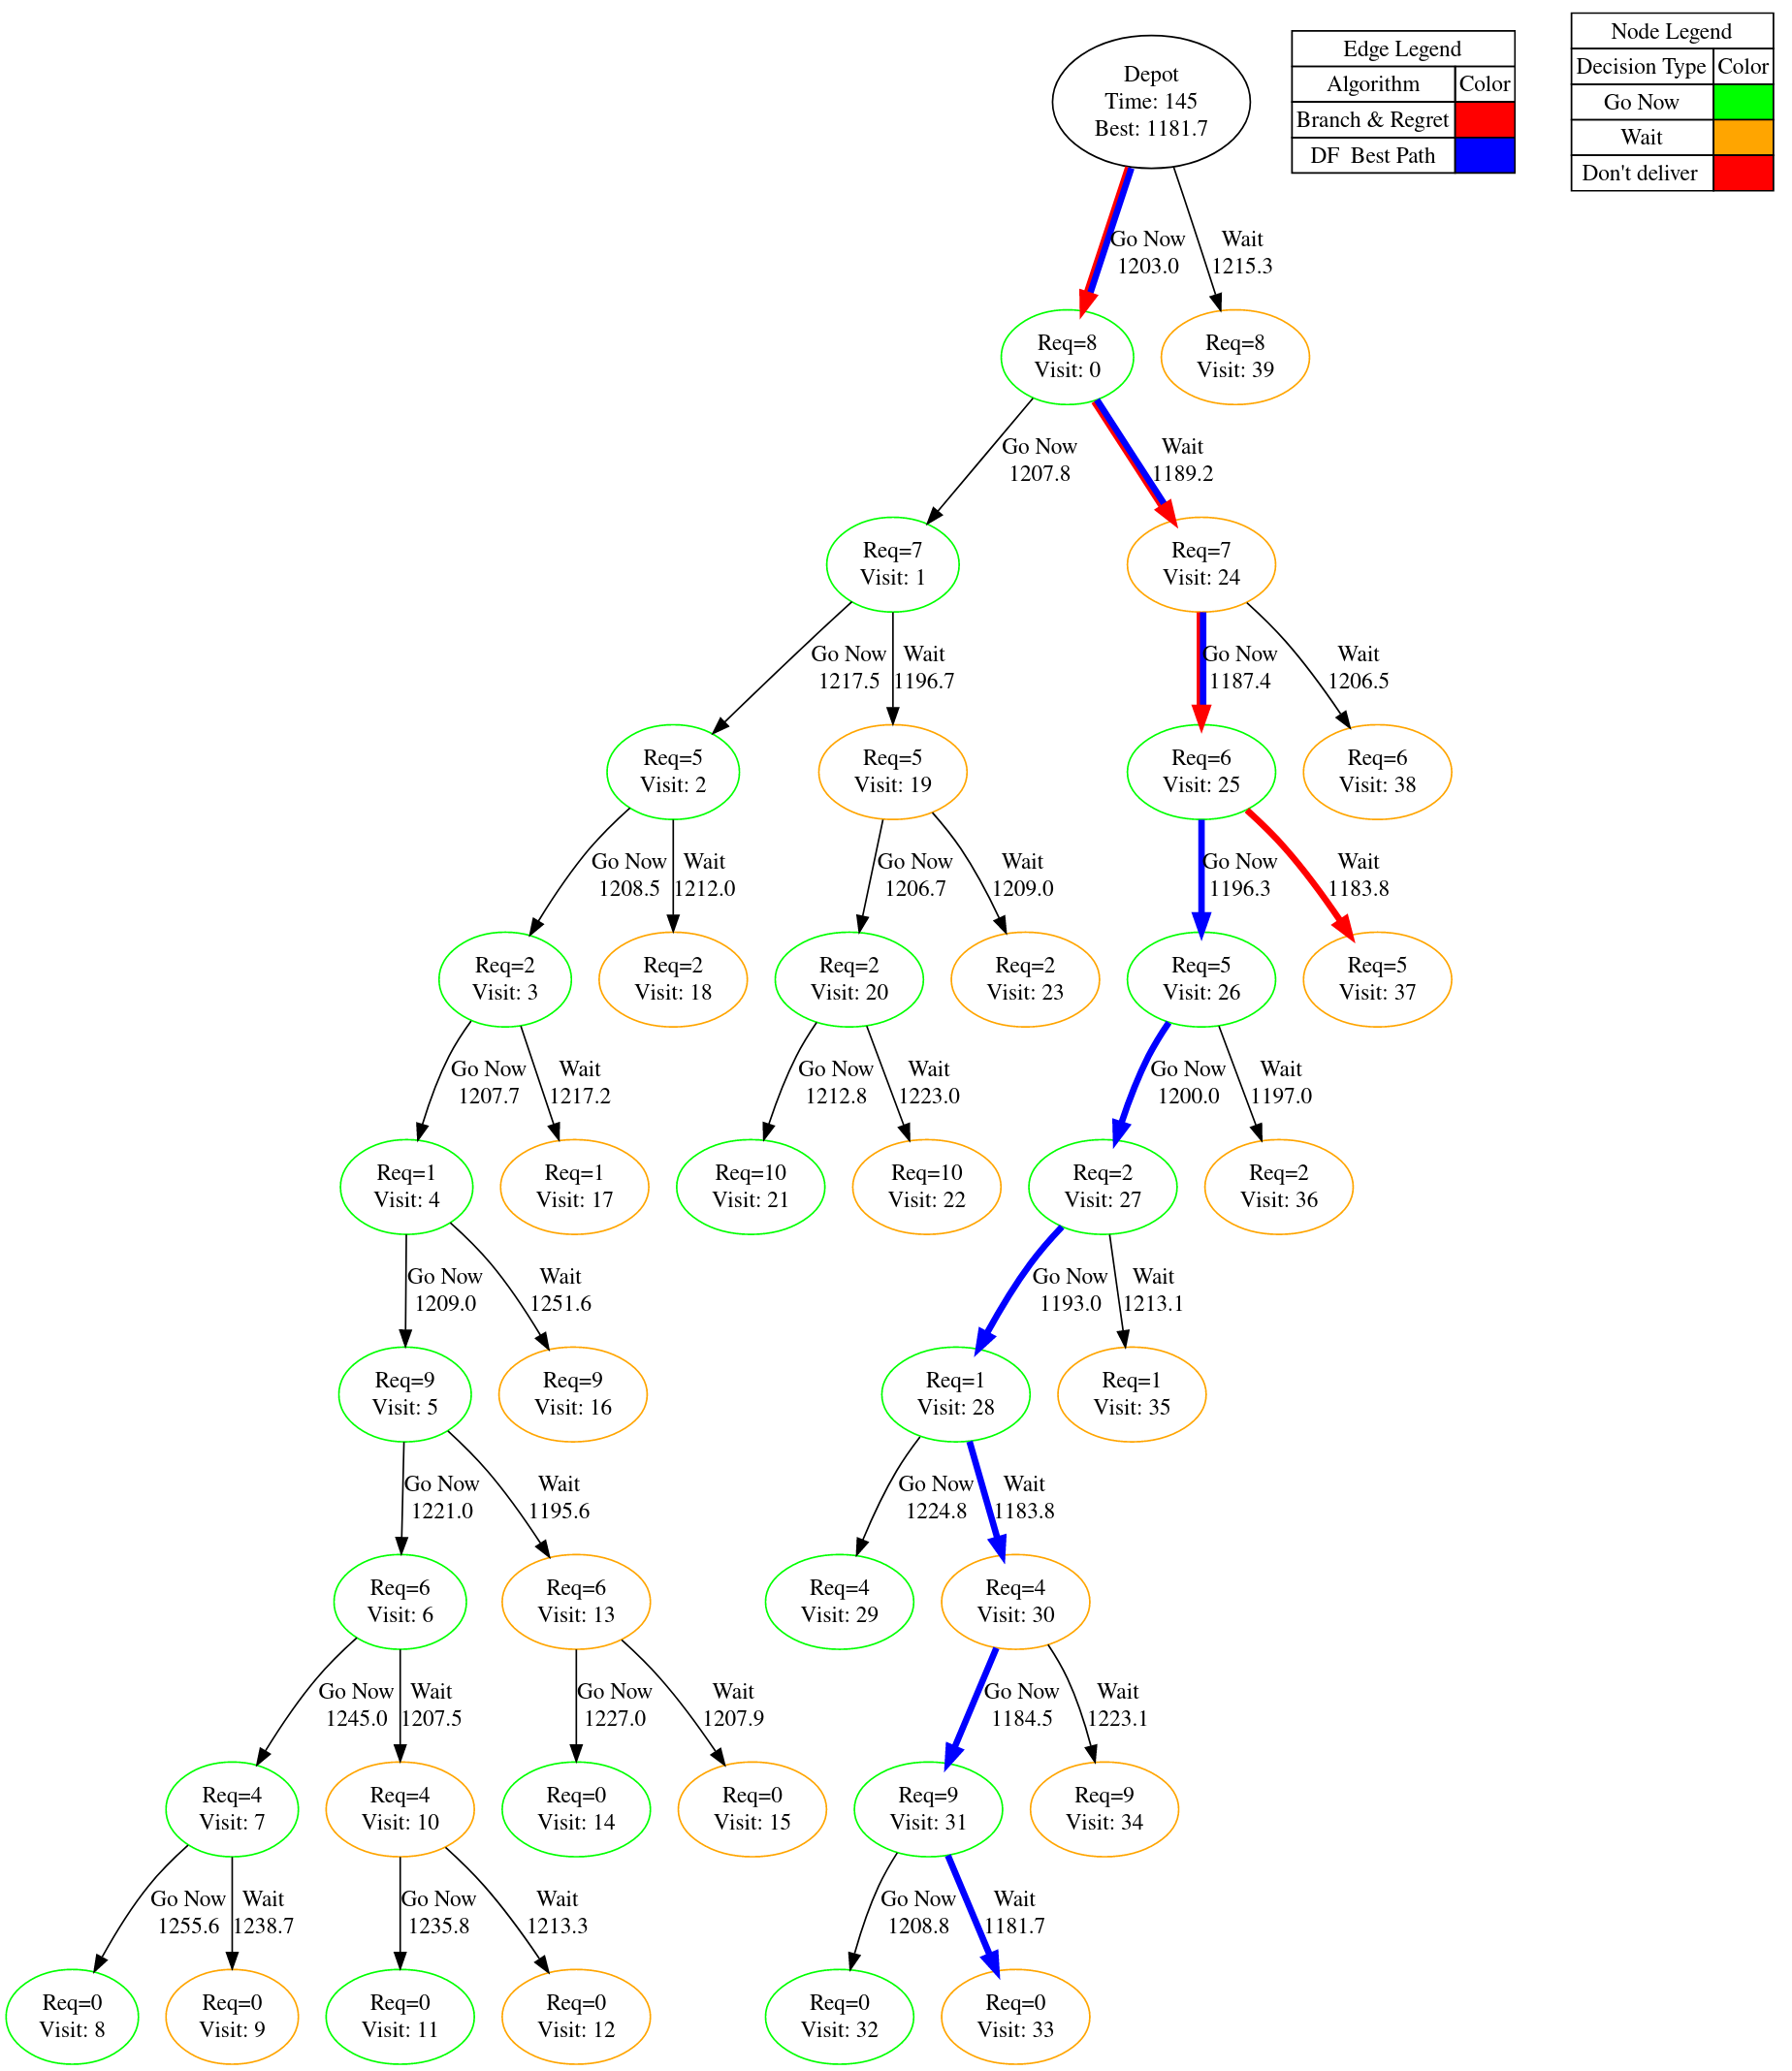
\includegraphics[width=0.7\textwidth]{Images/good_shit.png}
                \caption{B\&B Dept-First trova un percorso migliore del B\&R}
                \label{fig:BBDFmigliore}
            \end{figure}
    \end{frame}
    
    \subsection{Considerazioni e Conclusioni}\label{sec:considerazioni-conclusioni}

    \begin{frame}{Considerazioni sull'esecuzione}
        Per mostrare e confrontare i risultati del B\&B da noi implementato con il B\&R di Jean-François è necessario accennare al fatto che nel codice l'algoritmo B\&B, esattamente come il B\&R, non viene chiamato nel caso in cui il piano preveda sole wait. Questa situazione che a primo avviso potrebbe sembrare rara capita invece circa il $90\%$ delle volte per semplici istanze. In questi casi il costo del B\&R coincide con il B\&B e le differenze tra i due algoritmi è pressocchè nulla. Vediamo ora invece le differenze tra i due algoritmi nel caso in cui la sequenza di azioni non sia composta da sole wait. Tutti i risultati che saranno mostrati prevede l'esecuzione di 100 iterazioni di ALNS, 30 scenari generati e 10 veicoli.
    \end{frame}

    \begin{frame}{Definizione Istanze}
        Le istanze che abbiamo usato per fare i test fanno parte del benchmark disponibile sul \href{https://sites.google.com/view/jfcote/}{sito di Jean-François}. Le istanze del problema vengono classificate in base a molte delle loro caratteristiche che vengono messe in successione nel nome del file stesso. Prendiamo come esempio di problema \texttt{TWdf\_C\_1\_hom\_1\_actual.txt} e proviamo a descrivere le sue caratteristiche:
        \begin{itemize}
            \item \textbf{TWdf}:
            \item \textbf{C\_1}:
            \item \textbf{hom\_1}:
            \item \textbf{actual}:
        \end{itemize}
    \end{frame}

    \begin{frame}{Istanze Usate}
        Sono state da noi considerate $810$ istanze eseguite sia con B\&B che con B\&R in modo che tenessero in considerazione una buona varietà di caratteristiche. Abbiamo preso tutti e i tre tipi principali \textbf{TWdf}, \textbf{TWh}, \textbf{TWh\_R} con varianti \textbf{C\_X}, \textbf{R\_X} e \textbf{RC\_X} con $1 \leq \textbf{X} \leq 9$. Di ognuno di questi tipi di istanze è stato fissato l'attributo \texttt{hom\_1}, strettamente correlato con la complessità del problema, e l'attributo \texttt{actual}.
    \end{frame}

    \begin{frame}{\texttt{runner.py}}
        La computazione è stata eseguita tramite uno script Python 3.10 (\texttt{runner.py}), da noi sviluppato, sia sul Branch\&Bound con esplorazione Best-First, sia sul programma di Jean-François, per un totale di 1620 esecuzioni. Il tempo di calcolo per il B\&B è di \texttt{3443.94} secondi (circa \texttt{57} minuti), mentre il B\&R ha richiesto circa il doppio: \texttt{6571} secondi (circa \texttt{110} minuti). Dopo ogni computazione i risultati prodotti dai programmi vengono salvati in file \texttt{.txt}
    \end{frame}

    \begin{frame}{\texttt{extractor.py}}
        Una volta ottenuti i file di output, un altro script (\texttt{extractor.py}) utilizza Regex per leggere i files \texttt{.txt} e comprimere le uniche informazioni per noi utili presenti nelle stampe di output in un nuovo file \texttt{.csv}. Il risultato di questa fase ci permette di passare dai 1620 file di output, uno per ogni run, ad una sola tabella \texttt{csv} una per il B\&B e una per il B\&R, con le seguenti colonne: 
        \begin{itemize}
             \item \textbf{Problem}: Il nome del problema risolto
            \item \textbf{Instance}: Quale delle 30 istanze del problema è stata analizzata
            \item \textbf{Cost}: Il costo della migliore soluzione identificata
            \item\textbf{Dist}: La distanza totale da tutti i mezzi
            \item\textbf{Time}: Il tempo (in secondi) richiesto per completare la computazione
            \item \textbf{Events}: Il numero di eventi che si sono considerati
            \item \textbf{Skipped}: Il numero di eventi/piani saltati perché composti solo da attese (wait)
        \end{itemize}
    \end{frame}

    \begin{frame}{\texttt{analyzer.py}}
        Mostreremo ora alcuni grafici ottenuti da un terzo e ultimo script Python (\texttt{analyzer.py}) che abbiamo implementato che attraverso le librerie \textbf{pandas}, \textbf{numpy} e \textbf{matplotlib} ci ha permesso facilmente di confrontare i risultati compressi dallo script precedente.
        \newline Nei grafi che mostreremo ogni punto rappresenta la media calcolata su tutte le 90 istanze con le prime due caratteristiche del nome coincidenti. Ogni punto sarà plottato mostrando esplicitamente il valore dell'ordinata corrispondente con deviazione standard.
    \end{frame}

    \begin{frame}{Means Events}
        \begin{figure}[!h]
            \centering
            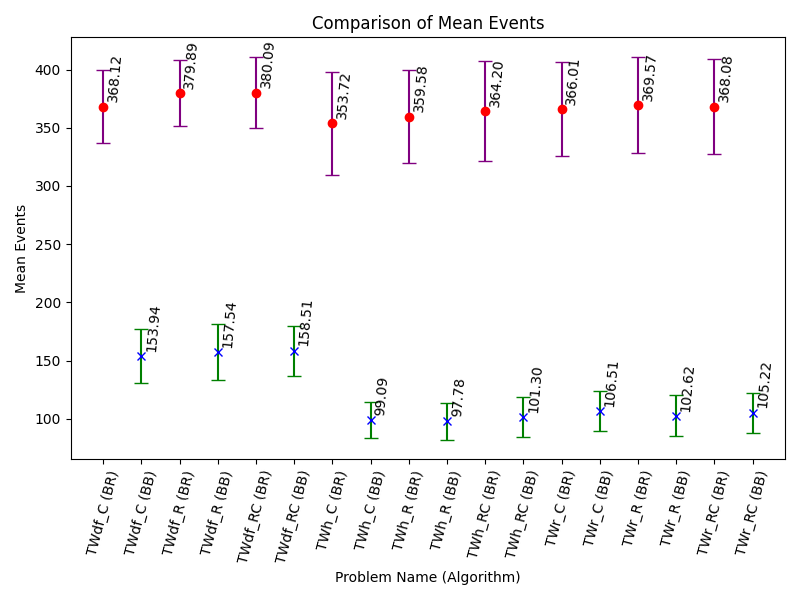
\includegraphics[width=0.82\textwidth]{Images/mean_events}
            \caption{B\&B vs B\&R: numero medio di eventi}
            \label{fig:mean_events}
        \end{figure}
    \end{frame}

    \begin{frame}{Mean Distance}
        \begin{figure}[h!]
            \centering
            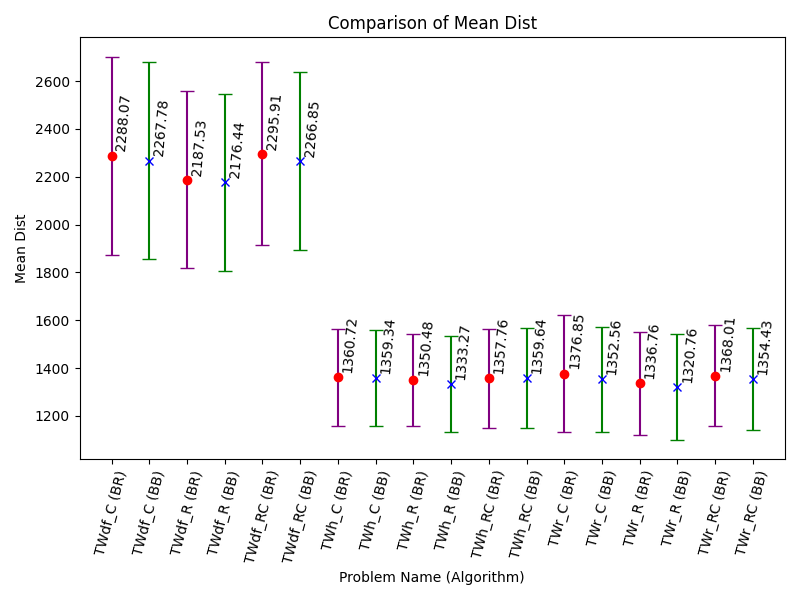
\includegraphics[width=0.82\textwidth]{Images/Mean_dist.png}
            \caption{B\&B vs B\&R: distanza media percorsa}
            \label{fig:Mean_dist}
        \end{figure}
    \end{frame}

    \begin{frame}{Mean Skipped}
        \begin{figure}[h!]
            \centering
            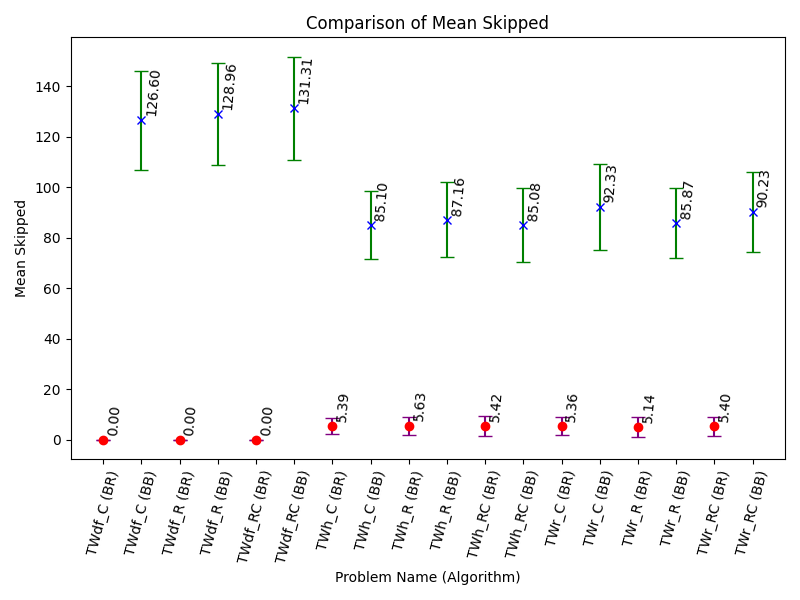
\includegraphics[width=0.82\textwidth]{Images/mean_skipped.png}
            \caption{B\&B vs B\&R: numero medio di eventi/piani saltati}
            \label{fig:mean_skipped}
        \end{figure}
    \end{frame}

    \begin{frame}{Mean Cost}
        \begin{figure}[h!]
            \centering
            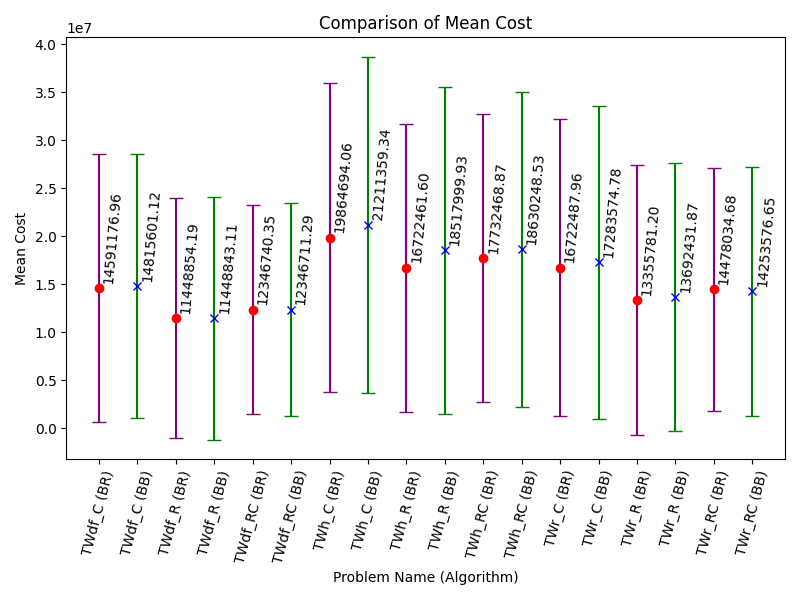
\includegraphics[width=0.82\textwidth]{Images/Mean_cost.png}
            \caption{B\&B vs B\&R: costo medio delle soluzioni}
            \label{fig:Mean_cost}
        \end{figure}
    \end{frame}

    \begin{frame}{Mean Time}
        \begin{figure}[h!]
            \centering
            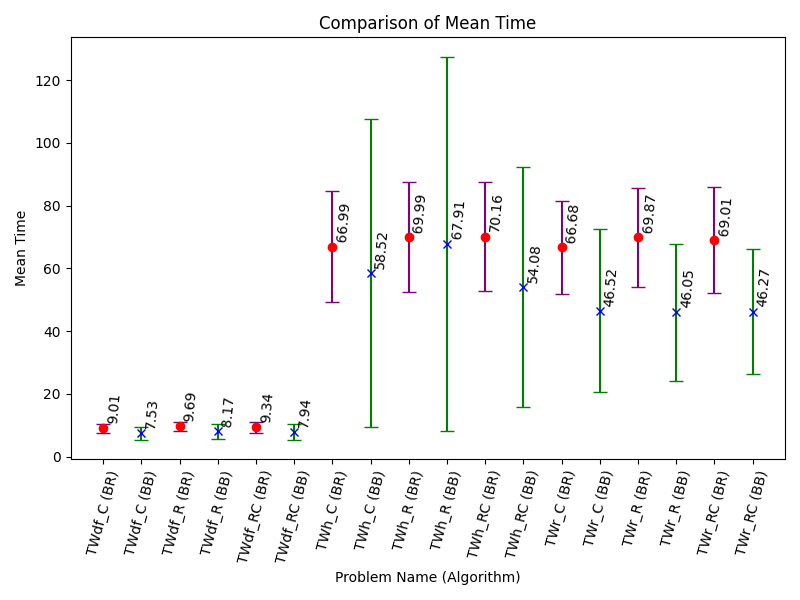
\includegraphics[width=1.0\textwidth]{Images/mean_time.png}
            \caption{B\&B vs B\&R: tempo medio necessario per completare la computazione}
            \label{fig:mean_time}
        \end{figure}
    \end{frame}
    
    \section*{Bibliografia}
    \begin{frame}{Bibliografia}
        \printbibliography[heading=none]
    \end{frame}
    
\end{document}